% vim: spell spelllang=en:
\documentclass[12pt, oneside]{article}
\usepackage[a4paper, left=2.5cm, right=2.5cm, top=2.5cm, bottom=2.5cm]{geometry}

\usepackage[utf8]{inputenc} % Use unicode
\usepackage[T1]{fontenc}
\usepackage[english]{babel} % Names in spanish

%% Bibliography:
%\usepackage{comment}
%\usepackage[
    %backend=biber,
    %style=numeric,
%]{biblatex}
%\DeclareNameAlias{default}{last-first}

%\usepackage{csquotes}       % For bibliography quotations
%\DeclareQuoteAlias{spanish}{catalan}

%\addbibresource{biblio.bib}
%% see:
%% https://www.sharelatex.com/learn/Bibliography_management_in_LaTeX#The_bibliography_file

%\usepackage{datetime} % Customize date
%% \monthyeardate\today gives the date without the day
%\newdateformat{monthyeardate}{%
    %\monthname[\THEMONTH], \THEYEAR}

% For cross references
\usepackage[colorlinks = true]{hyperref}
\usepackage[catalan]{varioref}
%\usepackage{cleveref}
%hyperref configuration so that it doesn't contrast so much colorlinks,
\hypersetup{
   linkcolor={black},
   citecolor={black},
   %linkcolor={red!50!black},
   %citecolor={blue!50!black},
   urlcolor={blue!80!black}
}

\usepackage{xcolor}     % color

\usepackage{mathtools}  % amsmath + more
\usepackage{amsthm}     % Theorem enviroment
\usepackage{amssymb}    % More symbols
\usepackage{amstext}    % Text inside mathenv

\usepackage{relsize}    % Bigger math with mathlarger{___}
\usepackage{nicefrac}   % nice fractions in one line

\usepackage[export]{adjustbox}  % Adjust table size
\usepackage{float}              % Force tables and images position (H and H!)
\usepackage{wrapfig}            % Wrap images like in HTML

\usepackage{tabularx, colortbl, booktabs}    % Better tables
\usepackage{longtable}                      % Multiple page table

% Split cell in lines and more formating options inside table
\usepackage{array, multirow, multicol, makecell}

%\usepackage{subcaption}                     % Subfigures
%\usepackage[framemethod=tikz]{mdframed}     % Custom frames

%\usepackage[bottom]{footmisc} % Footnotes at bottom of page

%\usepackage[alsoload=hep]{siunitx}          % SI units and uncertainties
%\sisetup{locale = FR}                       % Commas and so on for spanish
%\sisetup{separate-uncertainty=true}
%\sisetup{
  %per-mode=fraction,
  %fraction-function=\nicefrac
%}

%\usepackage{tikz}
%%\usetikzlibrary{arrows}
%%\usetikzlibrary{scopes}
%\usetikzlibrary{babel}

%\usepackage{listings}       % For code blocks

%% Custom code highlight
%\definecolor{codegreen}{rgb}{0,0.6,0}
%\definecolor{codegray}{rgb}{0.5,0.5,0.5}
%\definecolor{codepurple}{rgb}{0.58,0,0.82}
%\definecolor{backcolour}{rgb}{0.95,0.95,0.92}
%\definecolor{lightblue}{RGB}{135,206,250}

%\lstdefinestyle{mystyle}{ backgroundcolor=\color{backcolour},
    %commentstyle=\color{codegreen}, keywordstyle=\color{blue},
    %numberstyle=\tiny\color{codegray}, stringstyle=\color{red},
    %identifierstyle=\color{black}, basicstyle=\footnotesize,
    %%breakatwhitespace=false,
    %breaklines=true,
    %%captionpos=b,                    keepspaces=true,
    %numbers=left,                    numbersep=5pt,
    %showspaces=false,
    %%showstringspaces=false, showtabs=false,
    %tabsize=4
%}
%\lstset{style=mystyle}

\newcommand{\whitepage}{
    \clearpage\thispagestyle{empty}\addtocounter{page}{-1} \newpage \clearpage
}

% Add command before appendix session for page numbering: A-1
%\newcommand{\appendixpagenumbering}{
    %\break
    %\pagenumbering{arabic}
    %\renewcommand{\thepage}{\thesection-\arabic{page}}
%}

%% Custom Math operators (functions not in italic in math mode):
%\DeclareMathOperator{\arcsec}{arcsec}
%\DeclareMathOperator{\arccot}{arccot}
%\DeclareMathOperator{\arccsc}{arccsc}
%\DeclareMathOperator{\cis}{cis}


\usepackage[justification=centering]{caption}
\usepackage{subcaption}
\usepackage{graphicx}
\usepackage{enumitem}
\usepackage{lipsum}

\usepackage{siunitx}
\usepackage{hyphenat}

\usepackage{xcolor}

\definecolor{LightGray}{rgb}{0.83, 0.83, 0.83}
\definecolor{bg}{HTML}{282828}

\usepackage[newfloat]{minted}
\captionsetup[listing]{position=top}

\setminted{
style=monokai,
%frame=lines,
framesep=2mm,
baselinestretch=1.2,
breaklines,
bgcolor=bg,
fontsize=\footnotesize,
linenos
}

\renewcommand\theadfont{\bfseries}

\title{
    PAR Laboratory Assignment\\
    Lab 4: Divide and Conquer parallelism with OpenMP: Sorting
}

\author{
    par2109:
    Aleix Boné,
    Alex Herrero
}

\date{
    Spring 2019-20
}

\begin{document}

\thispagestyle{empty}
\clearpage
\setcounter{page}{-1}

\begin{titlepage}
{
    \centering
    \null
    \vfill
    {\Huge \bfseries PAR Laboratory Assignment\par}
    \vspace{3em}
    {\Large {\scshape Lab 4:} Divide and Conquer parallelism with OpenMP: Sorting \par}
    \vfill
\begin{center}
\end{center}
    \vspace{3cm}

    \vfill
    {\raggedleft \Large
        Aleix Boné\\
        Alex Herrero\\
        {\bfseries\ttfamily par2109}\\
        \vspace{4em}
        2020-05-15
        \par}
}
\end{titlepage}

\tableofcontents
\pagebreak

\section{Introduction}%
\label{sec:intro}

\subsection{Analysis with \emph{Tareador}}


% Include the relevant parts of the modified multisort-tareador.c code and comment where the calls to the Tareador API have been placed for each one of the two recursive task decomposition strategies considered.
\begin{listing}[H]
\inputminted[firstline=20,lastline=31]{c}{sources/multisort-tareador-leaf.c}
\inputminted[firstline=33,lastline=51]{c}{sources/multisort-tareador-leaf.c}
\caption{Calls to the tareador API added to multisort-tareador.c for the leaf task decomposition}
\label{listing:tareador_leaf}
\end{listing}

As we can observe in listing~\ref{listing:tareador_leaf} for the leaf task decomposition we added the \texttt{tareador\_start\_task()} and the \texttt{tareador\_end\_task()} in lines 23 and 25 respectively.

\begin{listing}[H]
\inputminted[firstline=20,lastline=31]{c}{sources/multisort-tareador-tree.c}
\inputminted[firstline=33,lastline=51]{c}{sources/multisort-tareador-tree.c}
\caption{Calls to the tareador API added to multisort-tareador.c for the tree task decomposition}
\label{listing:tareador_tree}
\end{listing}

In this case for tree task decomposition we added the \texttt{tareador\_start\_task()} in line 47 and the \texttt{tareador\_end\_task()} in line 49 as shown in the listing~\ref{listing:tareador_tree}.

% Comment also about the tasks graphs that are generated,
\begin{figure}[H]
\centering
%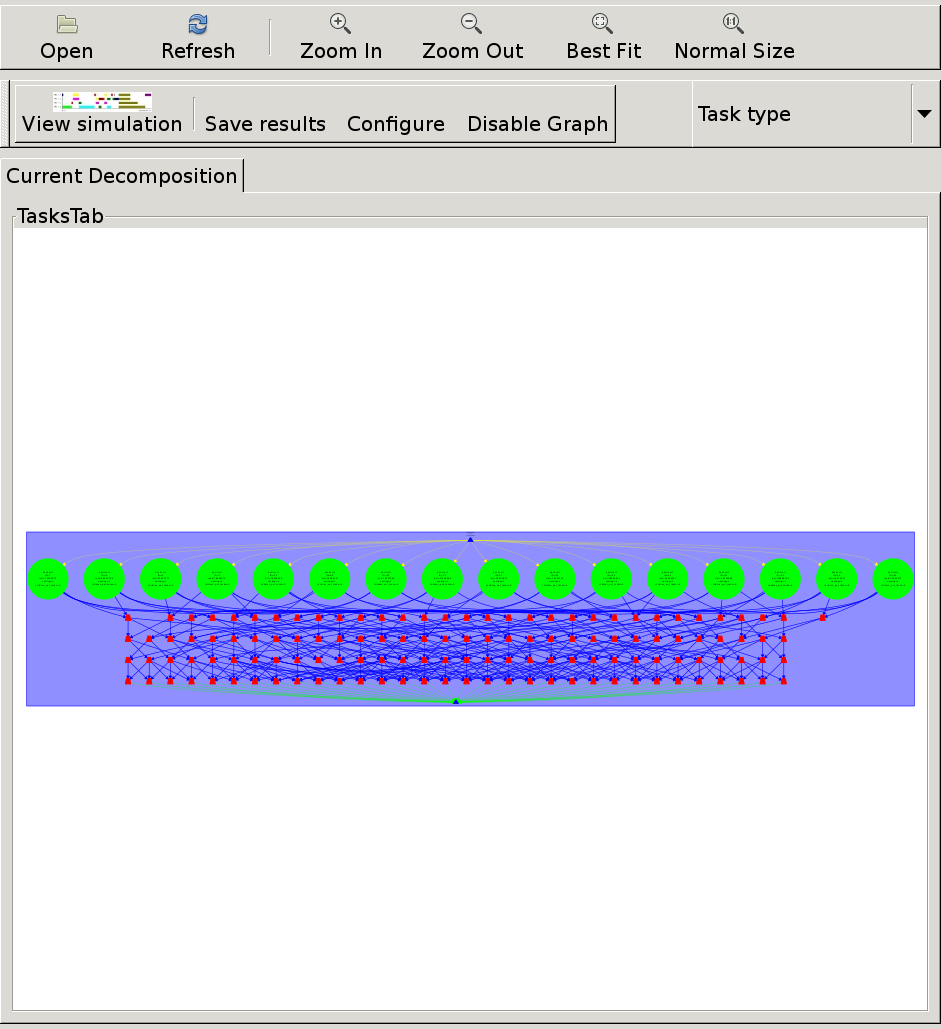
\includegraphics[width=0.8\textwidth]{captures/tareador-leaf.png}
\includegraphics[width=\textwidth]{dependency_graph_leaf.pdf}
\caption{Task dependence graph for leaf decomposition}
\label{fig:tar_tasks_leaf}
\end{figure}

\begin{figure}[H]
\centering
\includegraphics[width=0.8\textwidth]{dependency_graph_tree.pdf}
\caption{Task dependence graph for tree decomposition}
\label{fig:tar_tasks_tree}
\end{figure}

We also generated the task dependence graphs for both strategies (Figures~\ref{fig:tar_tasks_leaf} and~\ref{fig:tar_tasks_tree}).
% From the task dependence graphs that are generated, draw up a table showing the number of tasks doing computation (i.e.  those actually executing basicsort and basicmerge) and the number of internal tasks (i.e.  those that only create new tasks, basically executing invocations to multisort and merge) that are generated at each recursion level for each task decomposition strategy (having a clear explanation for the numbers on that table).
% including a table with the number of tasks that are generated at each recursion level for each task decomposition strategy.
\begin{table}[H]
\centering
\begin{tabular}{lrrrrr}
\toprule
Leaf strategy & & & & & \\
\midrule
Rec level:        & 1     & 2     & 3     & 4     & 5  \\
Tasks:    & 16    & 32    & 32    & 32    & 32 \\
\bottomrule
\end{tabular}

\caption{Number of tasks that are generated at each recursion level for leaf strategy} 
\label{tab:leaf_tasks-rec_level}
\end{table}

\begin{table}[H]
\centering
\begin{tabular}{lrrrrrrrrrrrrrrrrr}
\toprule
Tree strategy & & & & & & & & & & & & & & & & &\\
\midrule
Rec level:        & 1     & 2     & 3     & 4     & 5     & 6     & 7     & 8     & 9     & 10    & 11    & 12    & 13    & 14    & 15    & 16    & 17  \\
Tasks:    & 1     & 1     & 4     & 8     & 16    & 4     & 8     & 16    & 2     & 4     & 8     & 16    & 1     & 2     & 4     & 8    & 16 \\
\bottomrule
\end{tabular}

\caption{Number of tasks that are generated at each recursion level for tree strategy} 
\label{tab:tree_tasks-rec_level}
\end{table}

% You should also comment the task ordering constraints that have been identified and the causes for them, and the different kind of synchronisations that could be used to enforce them.
% TODO:

% For the analysis of scalability, include a table with the execution time and speed-up as predicted by Tareador(for 1, 2, 4, 8, 16, 32 and 64 processors).
\begin{table}[H]
\centering
\begin{tabular}{llrlr}
\toprule
           & Leaf strategy &           & Tree strategy &           \\
\midrule
Processors & Exec time (ms)& Speed-up  & Exec time (ms)& Speed-up  \\
\midrule
1          & 1.263.350     & 1,0000    & 1.263.350     & 1,0000    \\
2          & 631.688       & 2,0000    & 631.692       & 1,9999    \\
4          & 315.851       & 3,9998    & 316.452       & 3,9922    \\
8          & 158.381       & 7,9767    & 158.824       & 7,9544    \\
16         & 79.788        & 15,8338   & 79.787        & 15,8340   \\
32         & 79.746        & 15,8422   & 79.744        & 15,8426   \\
64         & 79.746        & 15,8422   & 79.744        & 15,8426   \\
\bottomrule
\end{tabular}
\caption{Table with the execution time and speed-up as predicted by \emph{Tareador}} 
\label{tab:Exec_time-Speed-up}
\end{table}

% Are  the  results  close  to  the  ideal  case?
In the table~\ref{tab:Exec_time-Speed-up} we can observe the execution time and speed-up as predicted by \emph{Tareador} for both strategies. We can see that for 1 to 16 processors the speed-up is quite close to the ideal case, but when we arrive to 32 processors the speed-up curve flattens away from the ideal line.

%Any observable differences between both recursive task decomposition strategies (leaf and tree)?
As shown in the table, both strategies (leaf and tree) have no big differences neither in execution time nor in speed-up, but it should be noted that with a low number of processors, the leaf strategy is a bit faster than the tree one, and with many processors the opposite happens.

%Which is (are) the factor(s) that limit the scalability in this case
In this case, with a large number of processors the scalability is limited because a large overhead is generated due to task creation. %TODO: ESTO ES ASI?

\section{Parallelization strategies}%
\label{sec:par_strats}

We studied two approaches to paralellization, leaf and tree task decomposition. For the leaf decomposition, we
defined tasks at the last level of the recursion: before calling \texttt{basicmerge} and \texttt{basicsort}. The
code corresponding to this version can be seem in listing~\ref{listing:omp_leaf}. 

For the tree task decomposition
we had to take into account the dependencies between tasks that we found while doing the analysis with \empht{Tareador}. Those are that all tasks to \texttt{multisort} have to finish before calling the corresponding
\texttt{merge}, and that the first two \texttt{merge} must finish before the last one. The code can be seen in
listing~\ref{listing:omp_tree}.

\begin{listing}[H]
\inputminted[firstline=32,lastline=63]{c}{sources/multisort-omp-leaf.c}
\caption{OpenMP pragmas added for leaf decomposition}
\label{listing:omp_leaf}
\end{listing}

\begin{listing}[H]
\inputminted[firstline=32,lastline=74]{c}{sources/multisort-omp-tree.c}
\caption{OpenMP pragmas added for tree decomposition}
\label{listing:omp_tree}
\end{listing}

In figures~\ref{fig:ssa_leaf} and \ref{fig:ssa_tree} we can observe the strong scalability analysis
of the leaf and the tree task decomposition respectively. It is clear from the plots that the
tree decomposition gives much better results than the leaf approach (which flattens out at around 5 threads).
Another fact to notice is that the speed-up of the multi-sort function has really good results, but the
whole application does not, this means that there are portions of the code outside of the multisort that are
affecting the performance noticeably.

\begin{figure}[H]
    \begin{minipage}{0.5\textwidth}
        \centering
        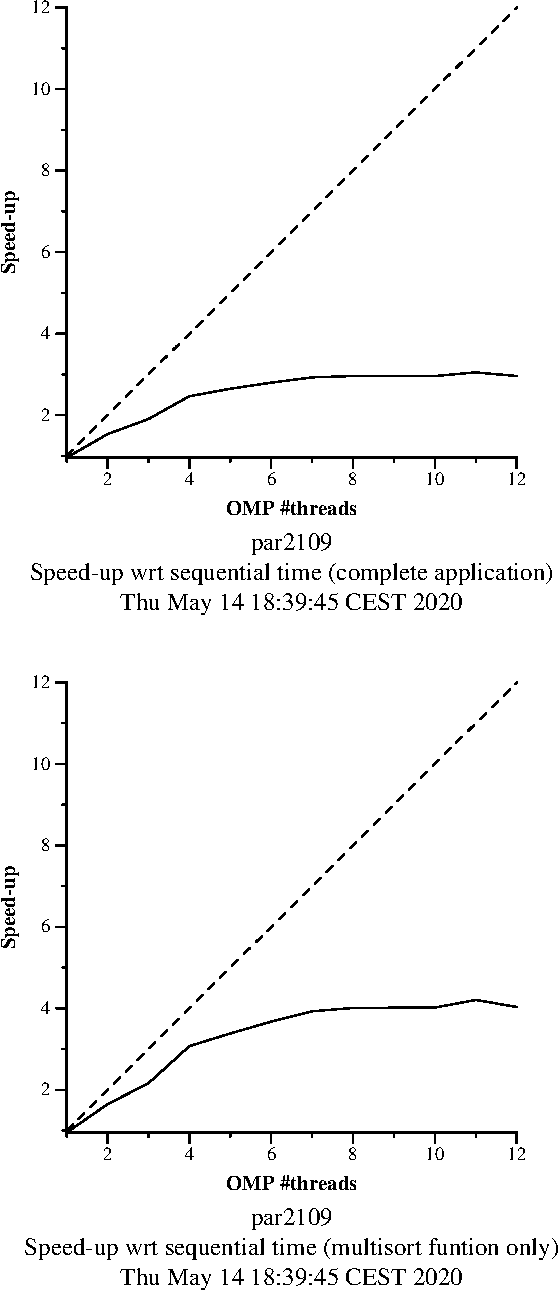
\includegraphics[width=0.7\linewidth]{plots/new-omp-leaf-crop.pdf}
        \caption{Strong scalability analysis leaf task decomposition}
        \label{fig:ssa_leaf} 
    \end{minipage}
    \begin{minipage}{0.5\textwidth}
        \centering
        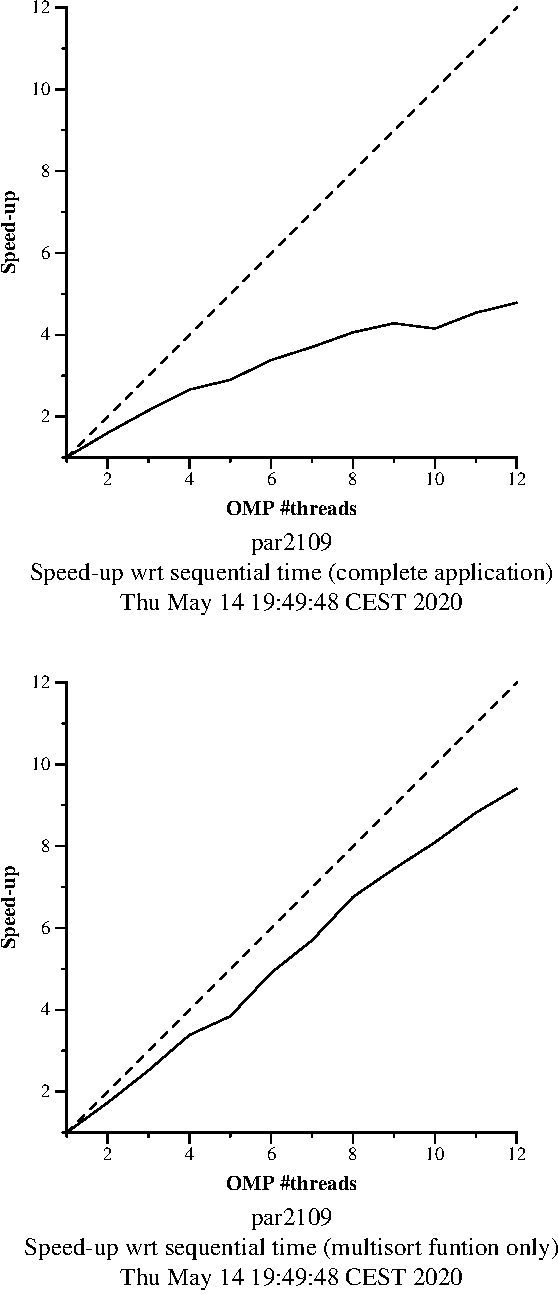
\includegraphics[width=0.7\linewidth]{plots/new-omp-tree-crop.pdf}
        \caption{Strong scalability analysis tree task decomposition}
        \label{fig:ssa_tree} 
    \end{minipage}
\end{figure}

\subsection{Cut-off}

To add a cut-off mechanism based on the recursion level, we added a parameter to the functions
\texttt{multisort} and \texttt{merge} called \texttt{depth} to keep track of the depth in the recursion.
With this parameter, we can add \texttt{final(depth > CUTOFF) mergeable} to the task pragmas to indicate
that once the depth is higher than the specified \texttt{CUTOFF} the next tasks should not be created.
The relevant parts of the code are shown in listing~\ref{listing:omp_tree_cutoff}.

\begin{listing}[H]
\inputminted[firstline=32,lastline=74]{c}{sources/multisort-omp-tree-cutoff.c}
\caption{OpenMP pragmas added for tree decomposition with cutoff}
\label{listing:omp_tree_cutoff}
\end{listing}

\begin{figure}[H]
    \begin{minipage}{0.5\textwidth}
        \centering
        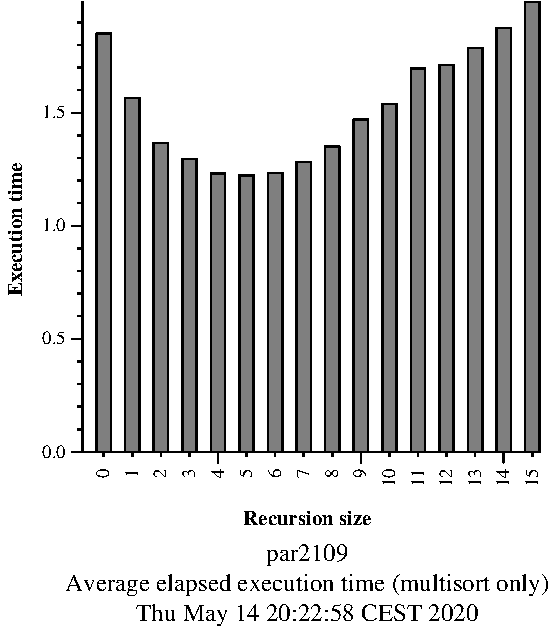
\includegraphics[width=0.7\linewidth]{plots/cutoff-8-crop.pdf}
        \caption{Cut-off 8 processors}
        \label{fig:cutoff8} 
    \end{minipage}
    \begin{minipage}{0.5\textwidth}
        \centering
        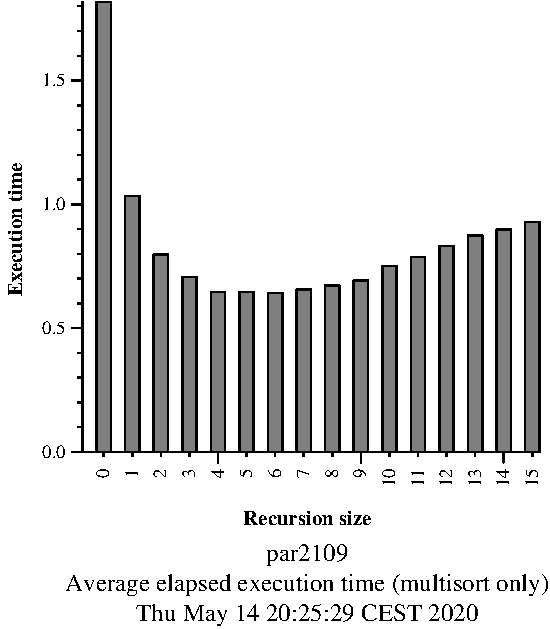
\includegraphics[width=0.7\linewidth]{plots/cutoff-24-crop.pdf}
        \caption{Cut-off 24 processors}
        \label{fig:cutoff24} 
    \end{minipage}
\end{figure}

As we can see in figures~\ref{fig:cutoff8} and \ref{fig:cutoff24}, the best results are obtained with a recursion
level of 5.

\begin{figure}[H]
    \begin{minipage}{0.5\textwidth}
        \centering
        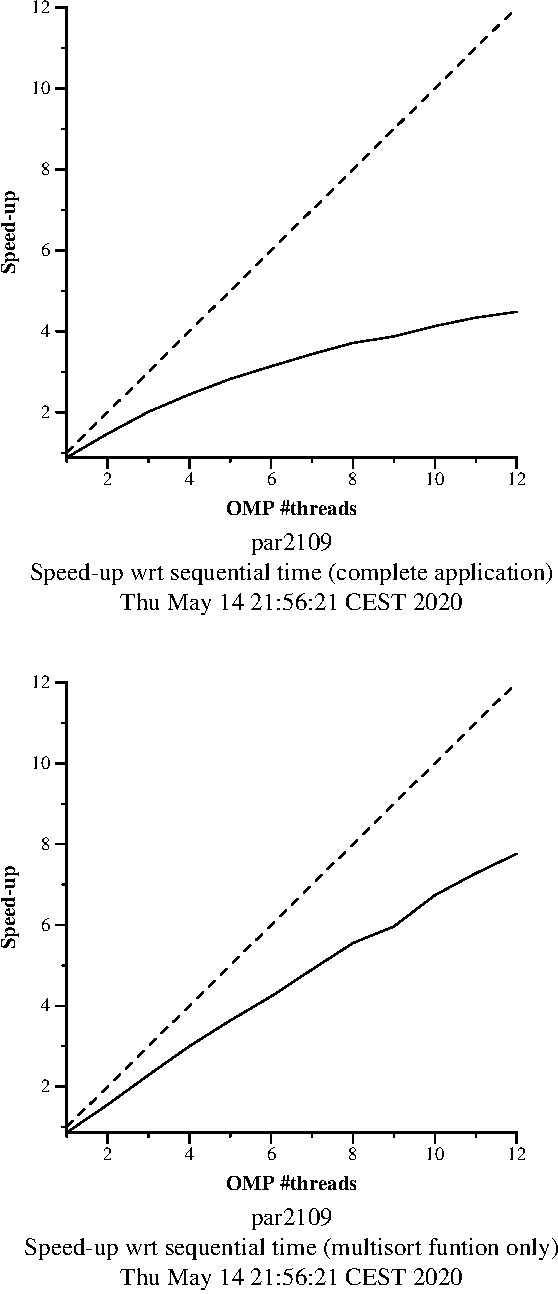
\includegraphics[width=0.7\textwidth]{plots/new-omp-tree-cutoff-5-crop.pdf}
        \caption{Scalability analysis with cutoff=5}
        \label{fig:cutoff5} 
    \end{minipage}
    \begin{minipage}{0.5\textwidth}
        \centering
        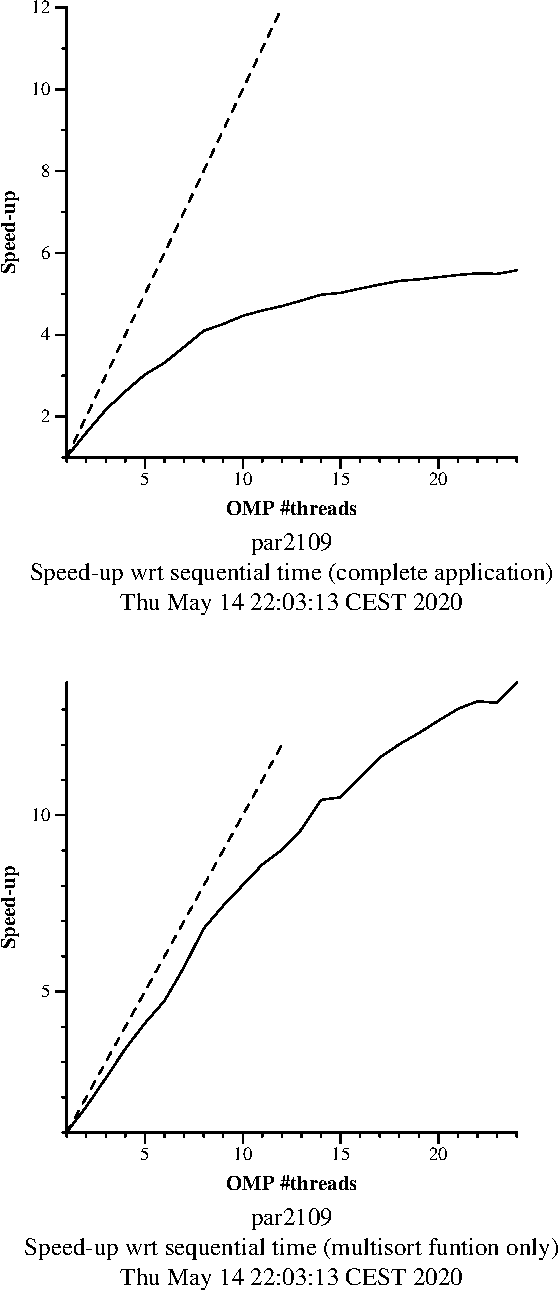
\includegraphics[width=0.7\linewidth]{plots/new-omp-tree-cutoff-24-crop.pdf}
        \caption{Scalability analysis with more than 12 threads}
        \label{fig:cutoff24} 
    \end{minipage}
\end{figure}

\begin{figure}[H]
    \begin{minipage}{0.5\textwidth}
        \centering
        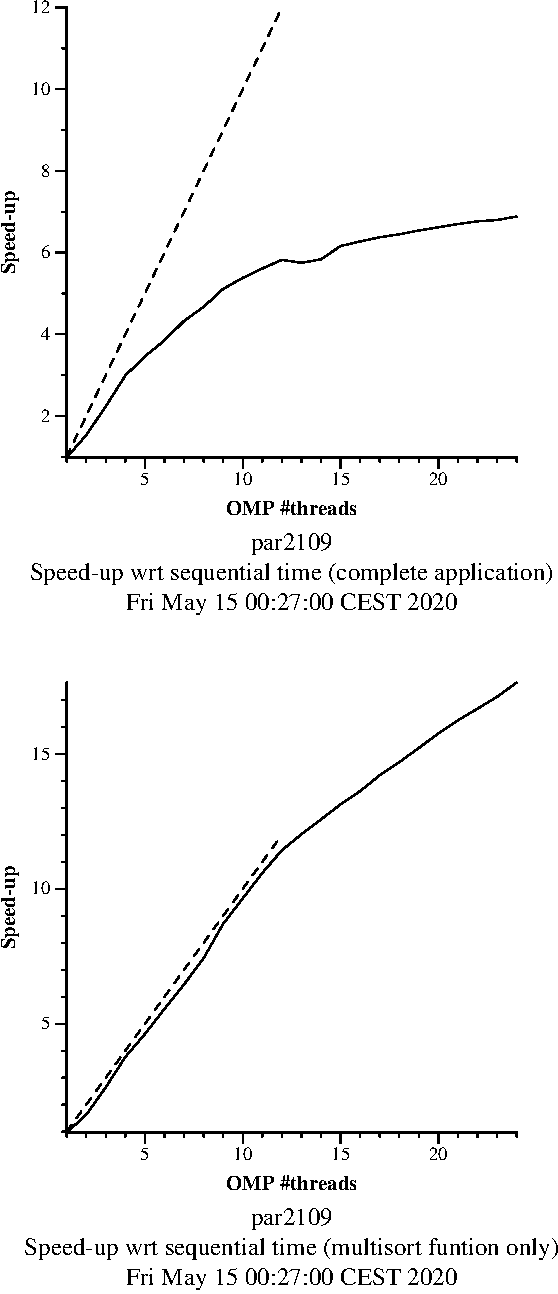
\includegraphics[width=0.7\linewidth]{plots/new-omp-tree-cutoff_boada5-crop.pdf}
        \caption{Scalability analysis on boada-5 (cuda)}
        \label{fig:cutoffboada5} 
    \end{minipage}
    \begin{minipage}{0.5\textwidth}
        \centering
        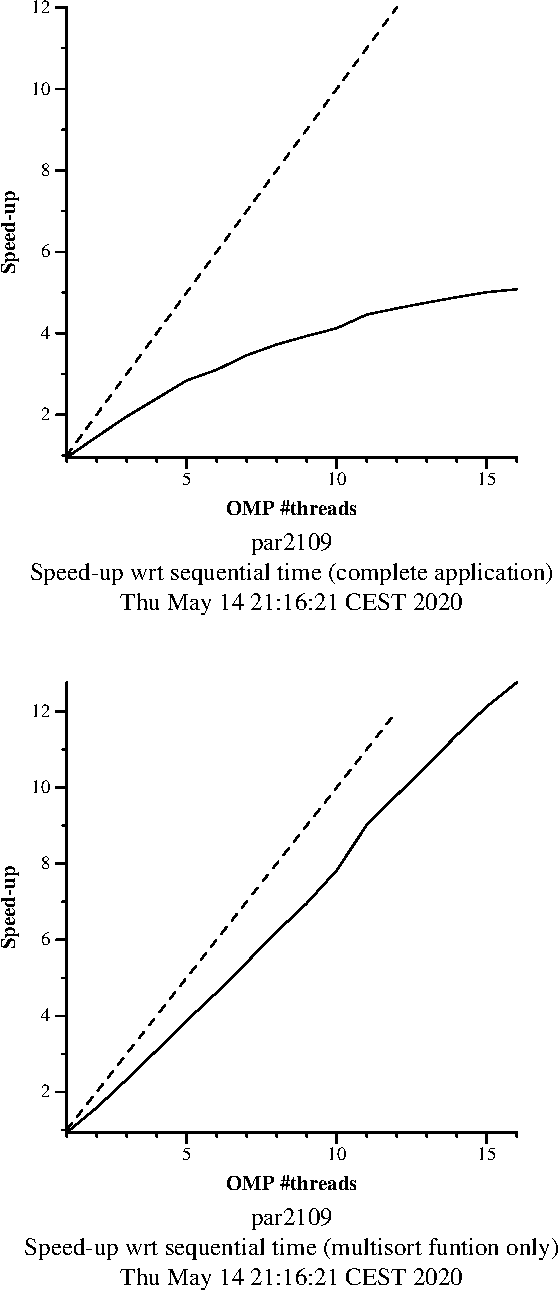
\includegraphics[width=0.7\linewidth]{plots/new-omp-tree-cutoff_boada7-crop.pdf}
        \caption{Scalability analysis on boada-7}
        \label{fig:cutoffboada7} 
    \end{minipage}
\end{figure}

If we analyze the traces of cutoff with values 0 and 1 with paraver, we can see that the execution time is reduced
from cutoff 0 to 1, but the time spent in scheduling and fork/join increases.


\begin{figure}[H]
    \begin{minipage}{0.5\textwidth}
        \centering
        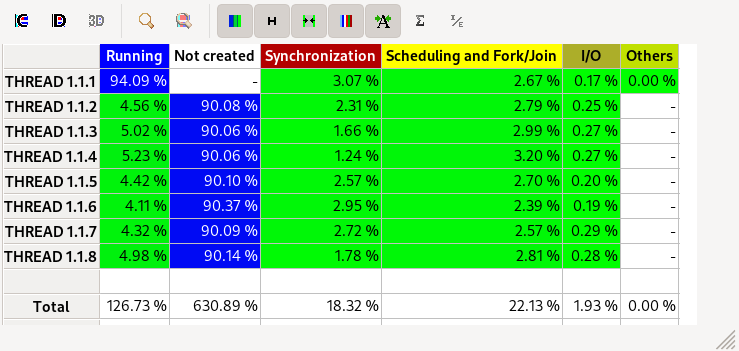
\includegraphics[width=0.7\linewidth]{captures/paraver_c0.png}
        \caption{Scalability analysis on boada-5 (cuda)}
        \label{fig:cutoffboada5} 
    \end{minipage}
    \begin{minipage}{0.5\textwidth}
        \centering
        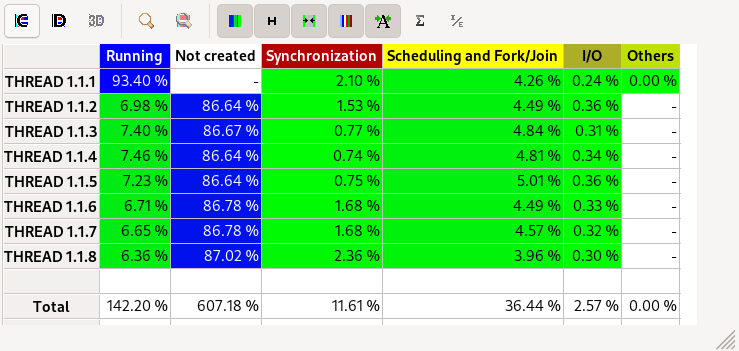
\includegraphics[width=0.7\linewidth]{captures/paraver_c1.png}
        \caption{Scalability analysis on boada-7}
        \label{fig:cutoffboada7} 
    \end{minipage}
\end{figure}

\subsection{Task dependencies}

Instead of using \texttt{taskgroup} and \texttt{taskwait} to manage the dependencies of the tasks we
explicitly declared the dependencies between them. We specified the initial position of the array for which
the tasks depended as show in listing~\ref{listing:omp_tree_depen}.

\begin{listing}[H]
\inputminted[firstline=32,lastline=71]{c}{sources/multisort-omp-tree-depen.c}
\caption{OpenMP pragmas added for tree decomposition with task dependencies}
\label{listing:omp_tree_depen}
\end{listing}

\section{Performance evaluation}%
\label{sec:perf_eval}

\section{Conclusions}%
\label{sec:conclusions}

\end{document}
